\documentclass[twocolumn]{article}

\usepackage{amsmath, amssymb} % Math formatting and symbols
\usepackage{graphicx} % Insert graphics
\usepackage{wrapfig} % Allow text to wrap around images
\usepackage[cm]{fullpage} % Smaller margins and header/footer
\usepackage{setspace}
\usepackage{gensymb} % degree symbol

\usepackage{float}

\usepackage{enumitem} % Allow for widest tag in enumerate

\usepackage{etoolbox}
\newcommand{\zerodisplayskips}{%
	\setlength{\abovedisplayskip}{0pt}%
	\setlength{\belowdisplayskip}{0pt}%
	\setlength{\abovedisplayshortskip}{0pt}%
	\setlength{\belowdisplayshortskip}{0pt}}
\appto{\normalsize}{\zerodisplayskips}
\appto{\small}{\zerodisplayskips}
\appto{\footnotesize}{\zerodisplayskips}

\renewcommand*\descriptionlabel[1]{\hspace\leftmargin$#1$}

\newenvironment{adescription}[1]
{\begin{list}{}%
		{\renewcommand\makelabel[1]{##1\hfill}%
			\settowidth\labelwidth{\makelabel{#1}}%
			\setlength\leftmargin{\labelwidth}
			\addtolength\leftmargin{\labelsep}}}
	{\end{list}}

\newcommand{\bd}{\textbf}
\newcommand{\dquad}{\quad{}\quad{}}

\title{\vspace{-5ex}Trigonometry \vspace{-5ex}}
\author{}
\date{}

\begin{document}
	\setstretch{1}
	\maketitle{}
	
	\subsection*{How to answer questions}
	
	Evaluate the trigonometric functions of the quadrant angle, if possible \\
	\indent -- Radians
	
	\noindent Reference Angle \\
	\indent -- Degrees/Radians will be specified \\
	\indent -- Always acute \\
	\indent -- Always positive \\
	\indent -- Between x-axis and terminal side
	
	\noindent Find two solutions of the equation. Give your answers in degrees ($ 0^\circ \le \theta < 360^\circ $) and in radians ($ 0 \le \theta < 2\pi $). Do not use a calculator. $ \sin(\theta) = -\frac{1}{2} $ \\
	\indent -- Always positive \\
	\indent -- Two answers \\
	\indent -- Exact values, draw circle
	
	\noindent Find the value of the expression, if possible $ \sin^{-1}(-\frac{\sqrt{3}}{2}) \text{ or}  \arcsin(-\frac{\sqrt{3}}{2}) $ \\
    \indent -- Radians assumed, unless specified otherwise \\
	\indent -- Exact = Picture, Round = Calculator \\
	\indent -- Positive or negative
	
	\subsection*{Basic Trigonometric Functions}
	\begin{align*}
		sin &= \frac{y}{r}  & csc &= \frac{r}{y} \\
		cos &= \frac{x}{r} & sec &= \frac{r}{x} \\
		tan &= \frac{y}{x} & cot &= \frac{x}{y}
	\end{align*}

	\begin{figure}[h]
		\centering
		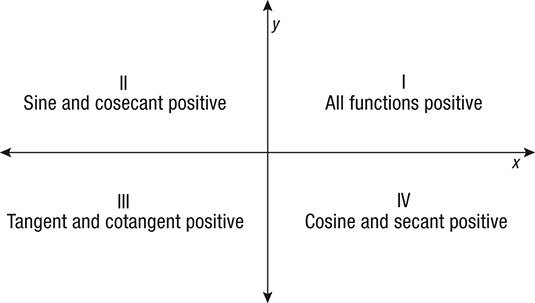
\includegraphics[width=0.25\textwidth]{positive_quadrants.jpg}
	\end{figure}

	\subsection*{Graphing Trigonometric Functions}

	Assume...
	\begin{itemize}[label=--]
		\setlength\itemsep{-0.55em}
		\item $ y = d + a * trig(bx - c) $
		\item Amplitude = $ \vert a \vert $
		\item Vertical Shift = $d$
		\item Phase Shift = $ \frac{c}{b} $
		\item X-Scale (change between critical points) = $ \frac{\text{period}}{4} $
		\item Period depends on what functions
		\item sin, cos, csc, sec = $ \frac{2\pi}{b} $
		\item tan, cot = $ \frac{\pi}{b} $
	\end{itemize}
	For deriving from a word problem
	\begin{itemize}[label=--]
		\setlength\itemsep{-0.55em}
		\item $ c = b * \text{shift} $
		\item b depends on what functions
		\item sin, cos, csc, sec = $ \frac{2\pi}{\text{period}} $
		\item tan, cot = $ \frac{\pi}{\text{period}} $
	\end{itemize}
	
	\subsubsection*{Examples...}

	\begin{figure}[H]
		\centering
		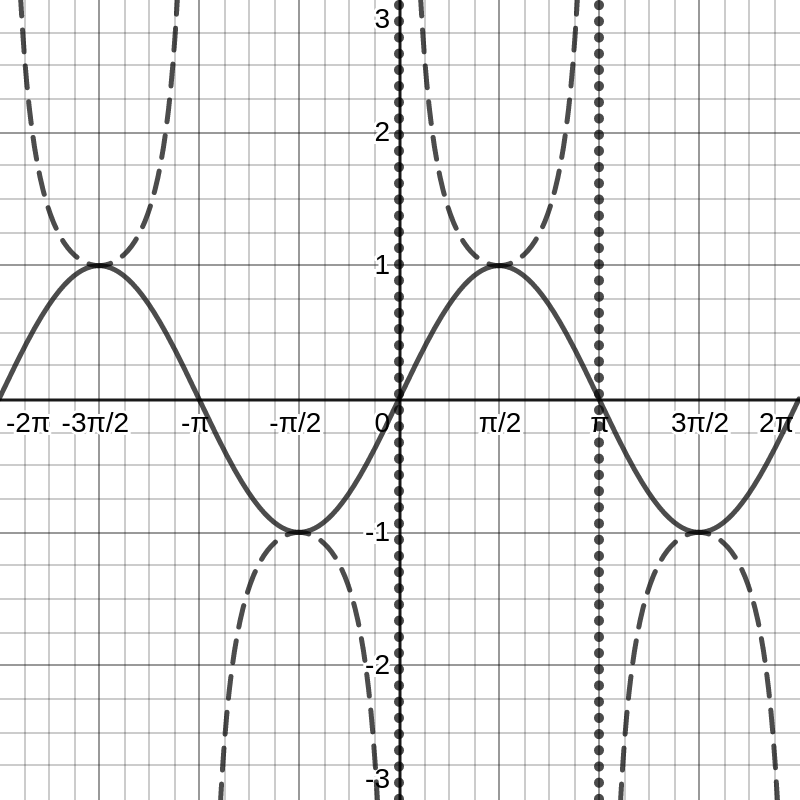
\includegraphics[width=0.20\textwidth]{sin-csc.png}
		\caption{$ y = \sin(x), y = \csc(x) $}
	\end{figure}

	\begin{figure}[H]
		\centering
		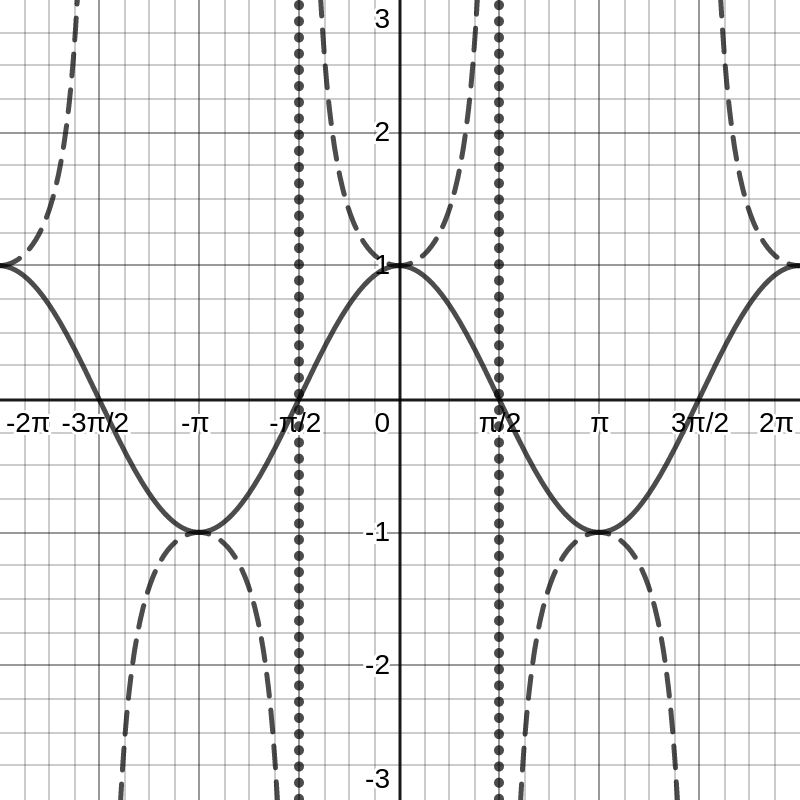
\includegraphics[width=0.20\textwidth]{cos-sec.png}
		\caption{$ y = \cos(x), y= \sec(x) $}
	\end{figure}

	\begin{figure}[H]
		\centering
		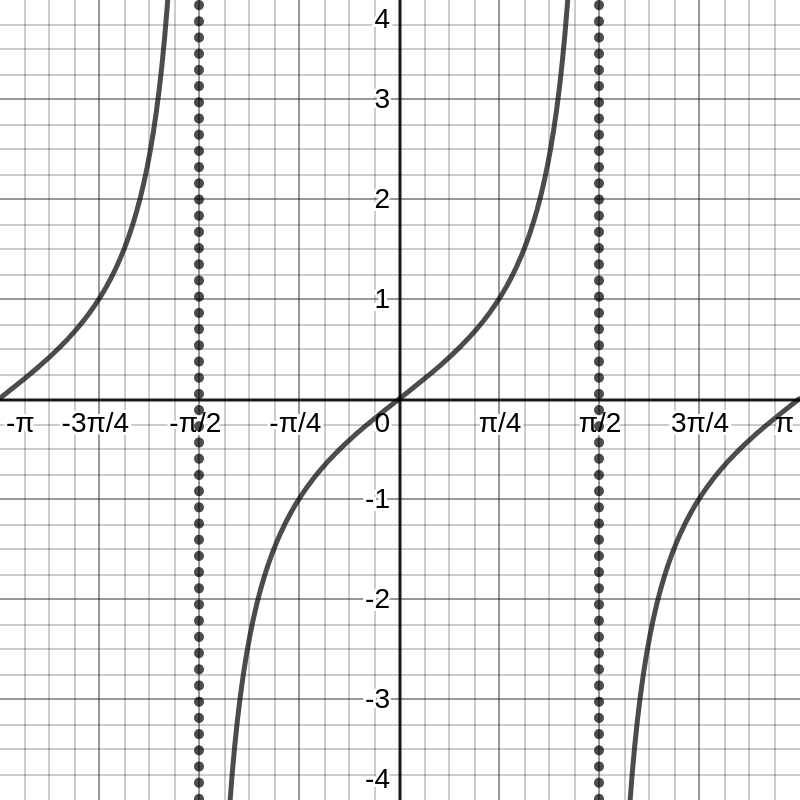
\includegraphics[width=0.20\textwidth]{tan.png}
		\caption{$ y = \tan(x) $}
	\end{figure}

	\begin{figure}[H]
		\centering
		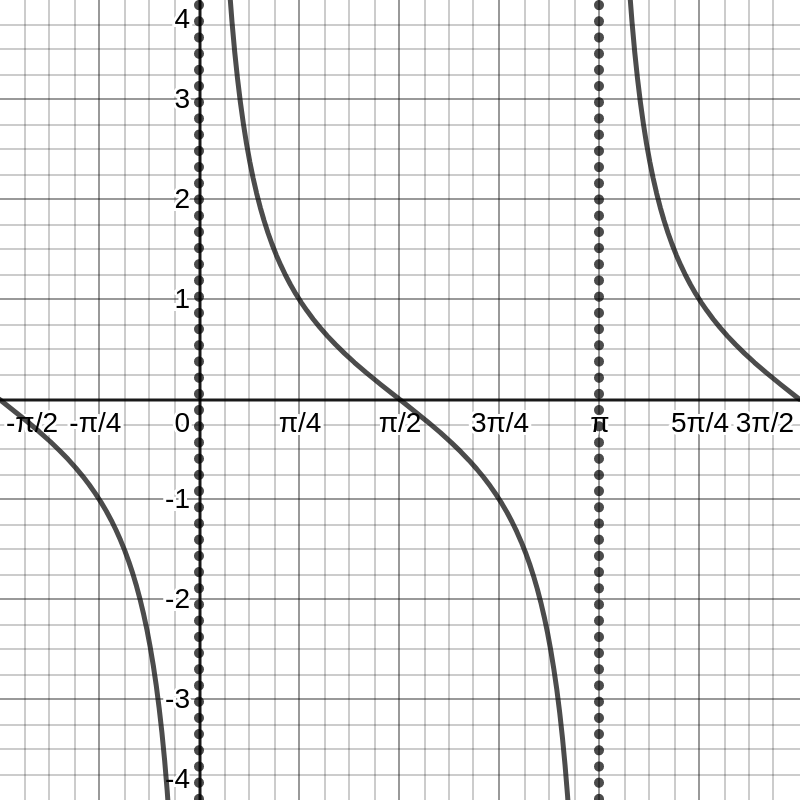
\includegraphics[width=0.20\textwidth]{cot.png}
		\caption{$ y = \cot(x) $}
	\end{figure}

	\subsection*{Trigonometric Identities}
	
	\begin{align*}
		\sin &= \frac{1}{\csc}  & \csc & = \frac{1}{\sin} \\
		\cos &= \frac{1}{\sec} & \sec & = \frac{1}{\cos} \\
		\tan &= \frac{\sin}{\cos}  & \cot & = \frac{\cos}{\sin}
	\end{align*}
	\vspace{0pt}
	\begin{align*}
		\sin^2 + \cos^2 &= 1 \\
		1 + \tan^2 &= \sec^2 \\
		1 + \cot^2 &= \csc^2
	\end{align*}
	\vspace{-2.2em}
	\subsection*{Arcs}
	In \bd{radians} unless specified otherwise \\
	Exact $\implies$ picture \\
	Round $\implies$ calculator ($\sin^{-1}$)
	
	\begin{align*}
		\sin(\theta) = -\frac{\sqrt{3}}{2} \\
		\sin^{-1}(-\frac{\sqrt{3}}{2}) \\
		 \arcsin(-\frac{\sqrt{3}}{2})
	\end{align*}

	\begin{figure}[H]
		\centering
		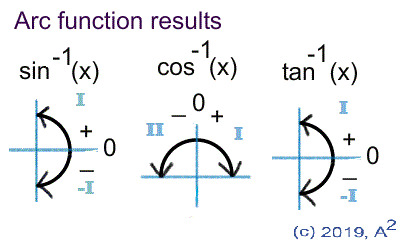
\includegraphics[width=0.20\textwidth]{ArcTrig.jpg}
	\end{figure}

\end{document}